% DAFN - ROS 2 - Lecture 2: Advanced Communication
% Roberto Masocco <roberto.masocco@uniroma2.it>
% April 21, 2022

\documentclass{beamer}

% Slides layout
\usepackage[
    title={Robot Operating System 2},
    subtitle={Lecture 2: Advanced Communication},
    event={DAFN},
    author={Roberto Masocco},
    longauthor={Roberto Masocco},
    email={roberto.masocco@uniroma2.it},
    institute={Tor Vergata},
    longinstitute={University of Rome "Tor Vergata"},
    department={Department of Civil Engineering and Computer Science Engineering},
    researchgroup={Intelligent Systems Lab},
    date={April 28, 2022}
]{utvengbeamer}

% Code listings settings
\usepackage[nomath]{lmodern}
\definecolor{codegreen}{rgb}{0 0.5 0}
\definecolor{codered}{rgb}{1 0 0}
\definecolor{codeocher}{rgb}{0.8 0.47 0.13}
\usepackage{listings}
\lstdefinestyle{beamer}{
    basicstyle=\ttfamily\small,
    commentstyle=\color{codegreen},
    breakatwhitespace=false,
    captionpos=b,
    frame=lines,
    keepspaces=true,
    keywordstyle=\color{codered}\bfseries,
    numbers=left,
    numbersep=5pt,
    numberstyle=\footnotesize,
    showspaces=false,
    showstringspaces=false,
    showtabs=false,
    stringstyle=\color{codeocher},
    tabsize=2
}
\lstset{style=beamer}
\lstdefinelanguage{ros2msg}{
  alsoletter={[, ], _, /},
  morecomment=[l][\color{codegreen}]{\#},
  morekeywords={int64, uint32, string, uint8, uint8[], int32, int32[] std_msgs/Header}
}

\usepackage{hyperref}
\usepackage{wasysym}

\begin{document}

% --- Title page ---
\frame{\titlepage}

% --- Table of contents ---
\begin{frame}
\frametitle{Roadmap}
\tableofcontents
\end{frame}

% --- Section 1 ---
% Section 1 - Services
% Roberto Masocco <roberto.masocco@uniroma2.it>
% April 21, 2022

% ### Services ###
\section{Services}
\graphicspath{{figs/section1/}}


% --- Section 2 ---
% Section 2 - Actions
% Roberto Masocco <roberto.masocco@uniroma2.it>
% April 21, 2022

% ### Actions ###
\section{Actions}
\graphicspath{{figs/section2/}}

% --- Services Limitations ---
\begin{frame}{Services Limitations}
The third paradigm exists because services implementation relies on the following \textbg{restrictive assumptions}.
\begin{alertblock}{Services Implementation Assumptions}
  \begin{itemize}
    \item Since the client may block for the entire duration of the request processing, \textbr{server computations should be short and always produce some result} (e.g. even an error must be a result).
    \item Service calls are finished only when the response has been received, i.e. \textbr{if either the client or the server crash, the behaviour of the other one is undefined} (say hello to deadlocks, crashes...).
    \item Once a service is called, \textbr{the request may never be interrupted}.
  \end{itemize}
\end{alertblock}
These make \textbg{processes} that \textbg{must be requested} and \textbg{take a long time} (for CPUs!) completely unfeasible.\\
Think of practically-interesting stuff such as \textbg{movement}, \textbg{navigation}...
\end{frame}

% --- ROS 2 Actions ---
\begin{frame}{ROS 2 Actions}
Built on services and message topics, they \textbg{decouple computations from middleware tasks}, thanks to the concepts of \textbg{goal}, \textbg{feedback} and \textbg{result}.\\
Their implementation is still a bit cumbersome, but are \textbg{extensively used for robot navigation and movement}.
\begin{figure}
  \centering
  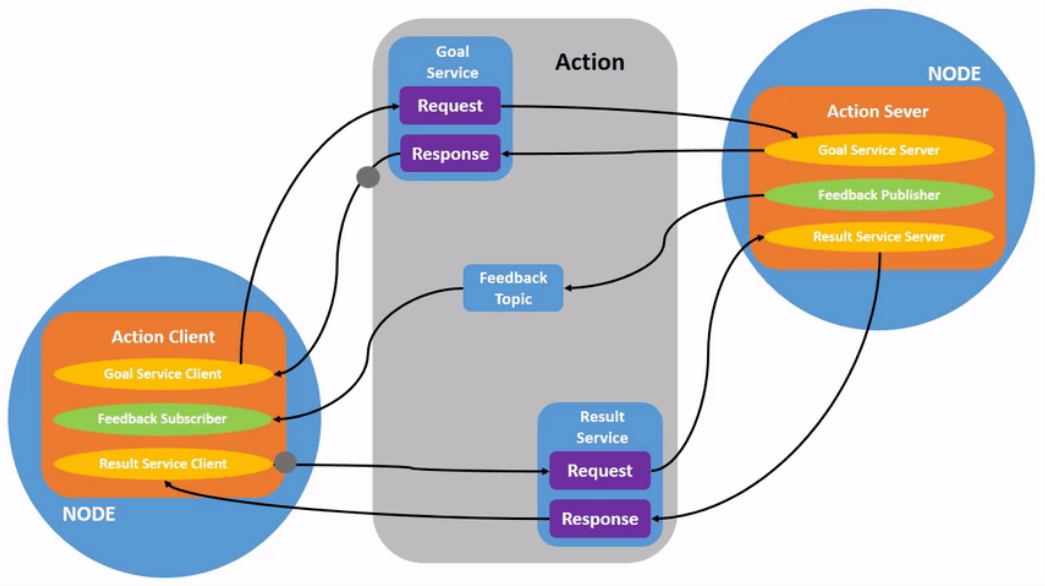
\includegraphics[scale=.31]{ros2Act.png}
  \label{fig:ros2Act}
  \caption{Example of an \emph{action server} and \emph{client}}
\end{figure}
\end{frame}
\begin{frame}{ROS 2 Actions}
\begin{figure}
  \centering
  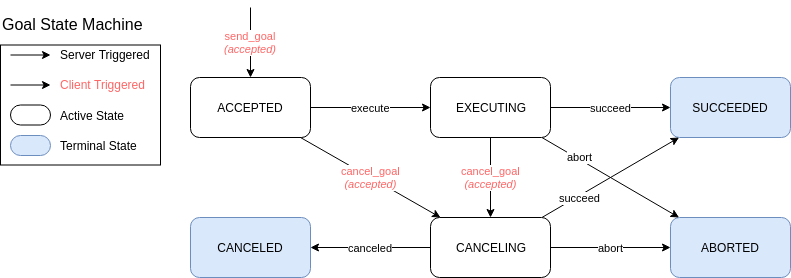
\includegraphics[width=\textwidth]{goalStateMachine.png}
  \label{fig:goalStateMachine}
  \caption{State machine\footnote{\href{http://design.ros2.org/articles/actions.html}{\color{blue}\underline{Actions - ROS 2 Design}}} of an action goal, managed by the middleware}
\end{figure}
\end{frame}
\begin{frame}{ROS 2 Actions}
In actual ROS 2 applications, the \textbg{client} requests the completion of some \textbg{goal} to the \textbg{server}. The middleware only offers APIs to \textbg{notify the state of the goal} between the two.
\begin{enumerate}
  \item The \textbg{client} sends a \textbg{goal service request} to the server.
  \item The \textbg{server} may \textbg{accept} or \textbg{reject} the goal request.
  \item Server computations, if any, are usually started when the goal is \textbg{executed}: the middleware only updates the state of the goal, the rest is up to the developer.
  \item The \textbg{client may cancel} the goal request; the \textbg{server may abort} the goal request; intermediate results and information, if any, are published by the server on the \textbg{feedback topic}.
  \item The \textbg{client} asks the server for the final result over the \textbg{result service}.
\end{enumerate}
\end{frame}

% --- Coding Action Servers and Clients ---
\begin{frame}{Coding Action Servers and Clients}
\begin{block}{Servers}
Goal requests are handled with \textbf{callbacks}, while computations can be handled freely (usually in separate threads). When done, the goal must be marked as \textbf{succeeded} or \textbf{aborted}, which triggers another callback to contact the client's result service.
\end{block}
\begin{block}{Clients}
Similarly to services, much is done with \textbf{\texttt{future} objects}. Cancellation request code can be placed almost everywhere and activated asynchronously.
\end{block}
Handling all possible scenarios for a goal results in the \textbg{longest and most complicated code that a ROS 2 application may ever require}. {\Large\smiley{}}
\end{frame}

% --- Interface Files - Actions ---
\begin{frame}[fragile]{Interface Files - Actions}
Combine \textbg{three messages} in a single interface file, separated by \texttt{-{}-{}-}.\\
Action file names end with \texttt{.action}.\\
There are no example packages for actions as of today.
\begin{columns}
\column{.9\textwidth}
% Listing: ros2_examples_interfaces/action/Fibonacci action definition
\begin{lstlisting}[language=ros2msg, caption=Definition of the \texttt{ros2\_examples\_interfaces/action/Fibonacci} action]
# GOAL
int32 order
---
# RESULT
int32[] sequence
---
# FEEDBACK
int32[] partial_sequence
\end{lstlisting}
\end{columns}
\end{frame}

% --- Example: Fibonacci Computer ---
\begin{frame}{Example: Fibonacci Computer}
Now go have a look at the \href{https://github.com/IntelligentSystemsLabUTV/ros2-examples/tree/galactic/src/actions_example}{\color{blue}\underline{ros2-examples/src/actions\_example}} package!
\end{frame}


\end{document}
